%!TEX root = ../thesis.tex

\chapter{Experiments}
\label{chap:pracPerf}
\section{Setup}
\label{sec:Setup}
In this chapter we will examine the practical relative performance of the three algorithms. We will do so in several ways. The first way is with the use of simulated data (recreated from \cite{Hastie2009}). We have ten features $X_1,\ldots,X_{10}$ which are drawn from a standard independent Gaussian. Their label is determined (deterministically) by the following rule: $$Y:=\begin{cases}
1 & \text{ if } \sum_{k=1}^{10} (X_k)^2 > \chi_{10}^2(0.5)\\
-1 & \text{otherwise}
\end{cases}$$ Where $\chi_{10}^2(0.5)=9.34$ is the median of a chi-squared random variable with ten degrees of freedom. This is to ensure that there are roughly the same number of labels in each category. 

\par The second way we will test the algorithms is the UCI ``a9a Adult data set'' \cite{LIBSVM}. Here the goal is to predict whether an individual will earn more than \$50,000 per year or not. The original data set has 14 features, among which six are continuous and eight are categorical. In this data set, continuous features are discretized into quantiles, and each quantile is represented by a binary feature. Furthermore a categorical feature with $m$ categories is converted to $m$ binary features. 

\par In an attempt to keep the comparison as consistent as possible we will, in all settings, use 32,561 observations for training and 16,281 for testing. This is because these are the number of observations in the a9a data set. This ratio of training to testing observations is not uncommon. Recall to avoid overfitting we cannot test the algorithm on the same data set we use for training. Thus any observations which are used to test cannot be used to train. Therefore this kind of ratio is desirable.

\par We implemented the algorithms in Python 3. Here we used Scikit-learn's implementation of a decision tree as our weak learner \cite{Pedregosa2012}. For the interested reader our implementations of all the algorithms discussed in this thesis, as well as everything necessary to recreate the experiments, is freely available at \url{https://github.com/dvente/bscthesis} 


\section{Results}
We will now discuss the results of our experiments in order to compare the algorithms.
\subsection{\adaB}
\label{subsec:AdaPracPerf}
\begin{figure}[!ht]
  \centering
      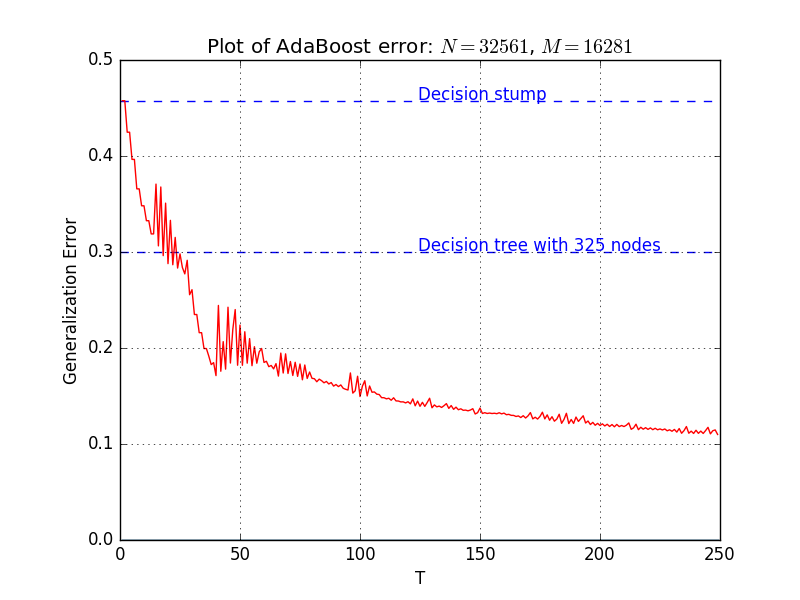
\includegraphics[width=\graphWidth]{generated/ADGD.png}
  \caption{Generalization error of AdaBoost as a function of the number of iterations over the simulated data set. The error rate of the decision stump and a decision tree with 325 nodes are shown for reference}
      \label{fig:adaBGD}
\end{figure}


\par Figure \ref{fig:adaBGD} shows the generalization error of \adaB as a function of the number of iterations on the simulated data set. Here we see it works as one would expect. The decision stump initially performs with an error rate of 47\% which is indeed only slightly better than random guessing. \adaB outperforms this and even a large tree with 325 nodes and an error rate of 30\% after just tens of iterations and reaches an error rate as low as 7.7\% after 500 iterations.

\newpage
\par Figure \ref{fig:adaBSVM} again shows the generalization error of \adaB as a function of iterations but this time over the a9a data set. Here the situation is somewhat different. One sees that the algorithm still works but here we run into some limitations. As we can see, the initial stump performs significantly better to start with, with an error rate of 23.6\%. After just 50 iterations we see diminishing returns set in quite drastically, seeing only a slight improvement from 15.7\% to 15.2\% over the course of 450 iterations. This also happens with the simulated data but to a much lesser degree. This is probably due to the fact that the simulated data is much more homogeneous, where in fact all features are equally important, with the difficult examples being those where all features are small but barely meet the criteria. The a9a data however most likely has a few features that considerably improve the accuracy (for example education), but beyond that, the data does not show any important examples so that the gains, after the low-hanging fruits have been picked, are marginal. While this is still a good result it is useful to keep this phenomenon in mind while we examine the remaining algorithms. This characteristic highlights a fundamental disadvantage of a weak learner, namely that depending on the data set there might simply not be a way to improve the accuracy beyond a certain point. 

\par A final observation on the reference trees should be useful here: while we tried to keep the size of the trees as consistent as possible, it is quite difficult to enforce a specific size over different data sets, especially ones that differ as strongly as our two data sets do. This is why the  trees have slightly different sizes across the different plots. We attempted to keep the sizes as similar as possible by enforcing a maximum depth of $\lfloor \log_2(500)\rfloor=8$, letting the algorithms fit the trees as best possible under this constraint. We have chosen this because it ensures an upper bound of 500 nodes, which we found to be a reasonable bound for the size and the shapes of our considered data.
\begin{figure}[!ht]
  \centering
      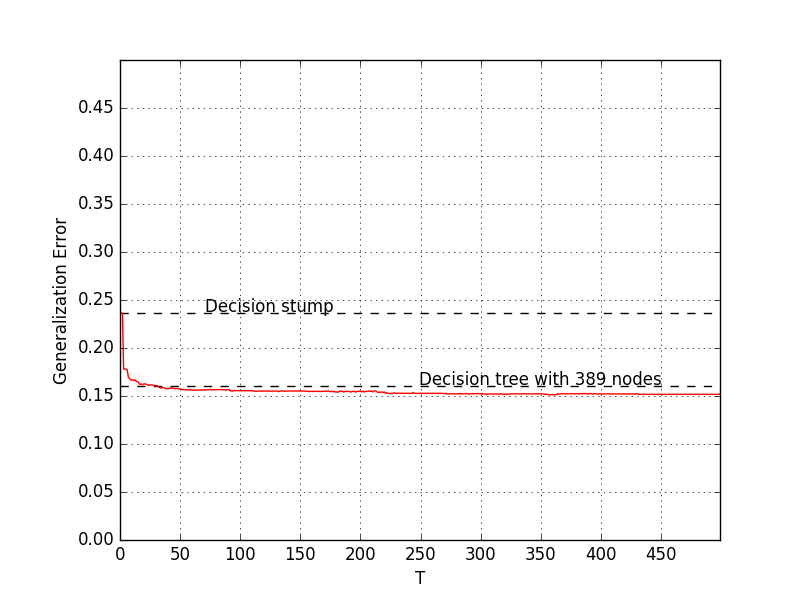
\includegraphics[width=\graphWidth]{generated/ADSVM.png}
  \caption{Generalization error of AdaBoost as a function of the number of iterations over the a9a data set. The error rate of the decision stump and a relatively large decision tree are again shown for reference}
      \label{fig:adaBSVM}
\end{figure}
\FloatBarrier

 \subsection{\NHB}
 \label{subsec:NHPracPerf}
Before we discuss the results of \NHB here we would like to highlight two important differences between \NHB and \adaB. The first is that to improve performance \NHB attempts to assign zero weight to unimportant examples in order to improve performance. The percentage of examples which were assigned weight zero is shown in green in the plots below. The second important difference is that whereas \adaB decides the label based on a reference threshold, \NHB simply takes an unweighted majority vote. A consequence of this is that on the even iterations the final committee might be tied on a decision. In an attempt to reflect this in our comparison we count the inconclusive tests (shown in a percentage of the testing size in blue) and recorded these as ``half a mistake'' since the committee was neither right nor wrong. Of course this impacts the performance of the algorithm quite significantly as can be seen below.  One important remark is that the committees are never tied in the case of an odd size. For the sake of clarity the graphs of the inconclusive tests in the plots below only show the percentage on the even iterations, those on the odd iterations always being 0.


\begin{figure}[!ht]
  \centering
      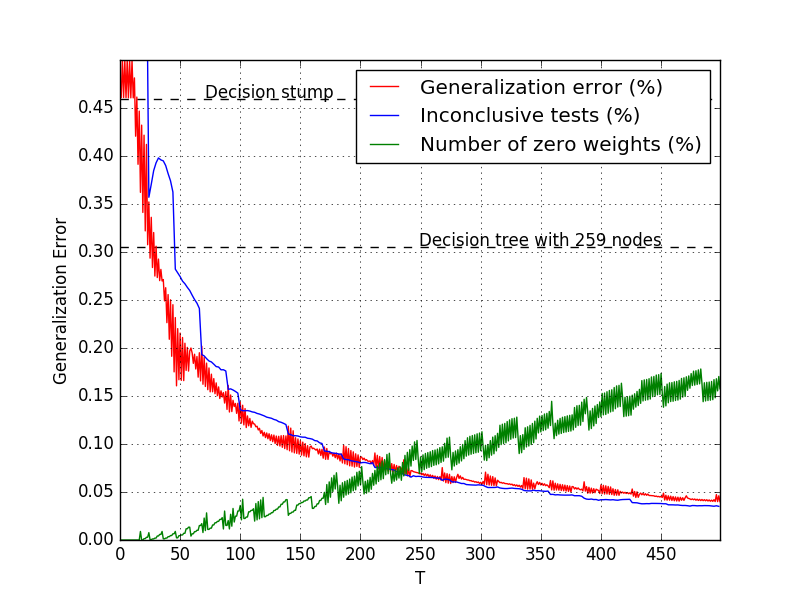
\includegraphics[width=\graphWidth]{generated/NHGD.png}
  \caption{Generalization error of \NHB as a function of the number of iterations on the simulated data. The error rates of trees with 3 and 259 nodes respectively are again shown for reference. It is important to remark that for the sake of clarity we omitted the inconclusive data points of all odd iterations as they are always 0.}
      \label{fig:NHBGD}
\end{figure}
 \FloatBarrier
 \par Here again figure \ref{fig:NHBGD} depicts the generalization error of \NHB as a function of the number of iterations on the simulated data set. The first thing one notices is that this mimics the behaviour predicted by the theory, as well as the behaviour of \adaB. The error rate as well as the percentage of inconclusive tests steadily declines whilst the percentage of zero weights steadily increases. In terms of actual percentages the algorithm performs quite well compared to \adaB. Where \adaB achieved an error rate of 7.7\% after 500 iterations \NHB achieves 3.9\% which is much better. This is achieved with a zero weight percentage of 15.7\% at the end. This, it should be noted, is a very significant portion. 
\begin{figure}[!ht]
  \centering
      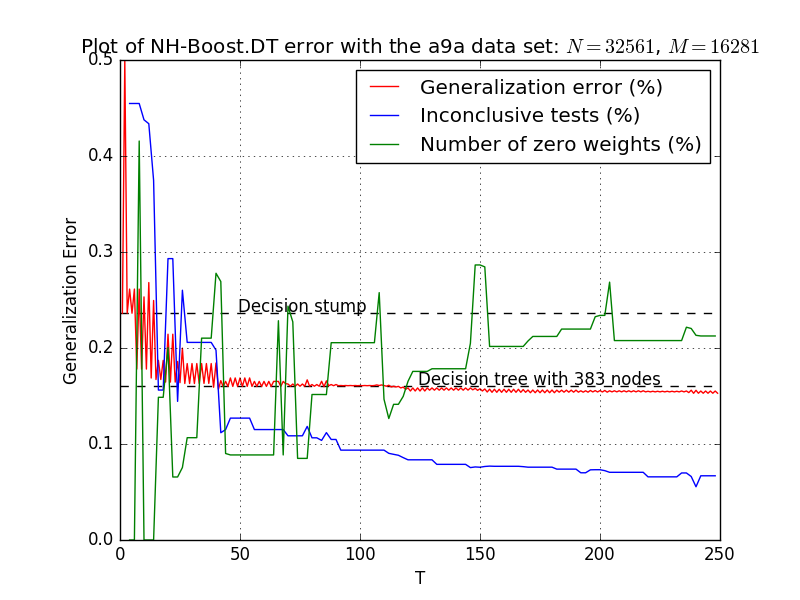
\includegraphics[width=\graphWidth]{generated/NHSVM.png}
  \caption{Generalization error of \NHB as a function of the number of iterations on the a9a data. The error rates of trees with 3 and 383 nodes respectively are again shown for reference. It is important to remark that for the sake of clarity we omitted the inconclusive data points of all odd iterations as they are always 0.}
      \label{fig:NHBSVM}
\end{figure}

\par When looking at the a9a data the situation is also a bit different. Figure \ref{fig:NHBSVM} again shows the generalization error of \NHB as a function of the number of iterations but over the a9a data set. The first obvious point to note when looking at figure \ref{fig:NHBSVM} is that the algorithm is (initially) quite confused about the number of examples to assign a zero weight. One possible cause is that the weights of the previous round are determined by the performance of the previous iteration and that the algorithm gets slightly confused by the inconclusive tests. The peaks of zero weights are almost all around the 28\% whereas the last iteration has a zero weight percentage of 23.2\%. This compares quite favourably to the previous data set, which can be explained by our interpretation that after the low hanging fruit has been picked many examples become irrelevant and thus get assigned zero weight. One can, however, also wonder how reliable this interpretation is due to all the peaks and valleys. 
\par Furthermore we again see the ``low-hanging fruit'' characteristics we saw in the \adaB implementation. Here the final error rate bottoms out at 15.1\% compared to \adaB 15.2\% which is almost identical. One can wonder about the role the inconclusive tests play in this conclusion. This is not however of great concern, since the accuracy on the odd iterations is also almost identical. Furthermore, the inconclusive tests are an indication that the committee is not certain on those predictions even when they are not tied in the odd iterations. This tells us that these percentages are indeed very comparable.  
\FloatBarrier
\subsection{\squintB}
\label{subsec:sqPracPerf}
Finally we will consider \squintB. Figure \ref{fig:SQGD} below shows the generalization error of \squintB as a function of the number of iteration over the simulated data set. Looking at it we again see the predicted behaviour. After a few initial spikes, both the error rate and the fraction of inconclusive tests steadily decline. As one can see it indeed performs somewhat similar to the other algorithms, finally achieving an error rate of 9.2\% compared to the 7.7\% and 3.9\% of \adaB and \NHB respectively. While it is still a good result, we conclude that \squintB performs worse than  \NHB and even \adaB. 
\begin{figure}[!ht]
  \centering
     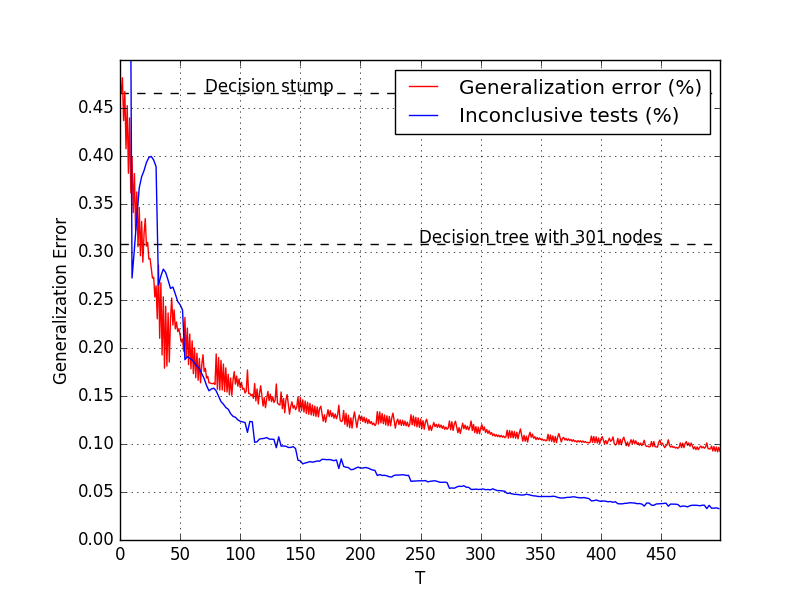
\includegraphics[width=\graphWidth]{generated/SQGD.png}
  \caption{Generalization error of \squintB as a function of the number of iterations on the simulated data. The error rates of trees with 3 and 301 nodes resp. are again shown for reference. It is important to remark that for clarities' sake we omitted the inconclusive data points of all odd iterations as they are always 0.}
      \label{fig:SQGD}
\end{figure}

\par Finally figure \ref{fig:SQSVM} depicts the generalization of \squintB as a function of the number of iterations over the a9a data set. When looking at it, we again see the same behaviour as with the other two algorithms. The initial improvement is quite fast but it bottoms out fairly quickly, finally achieving an error rate of 15.1\% which is again extremely similar to the 15.1\% and 15.2\% of the other two algorithms. 


\begin{figure}[!ht]
  \centering
    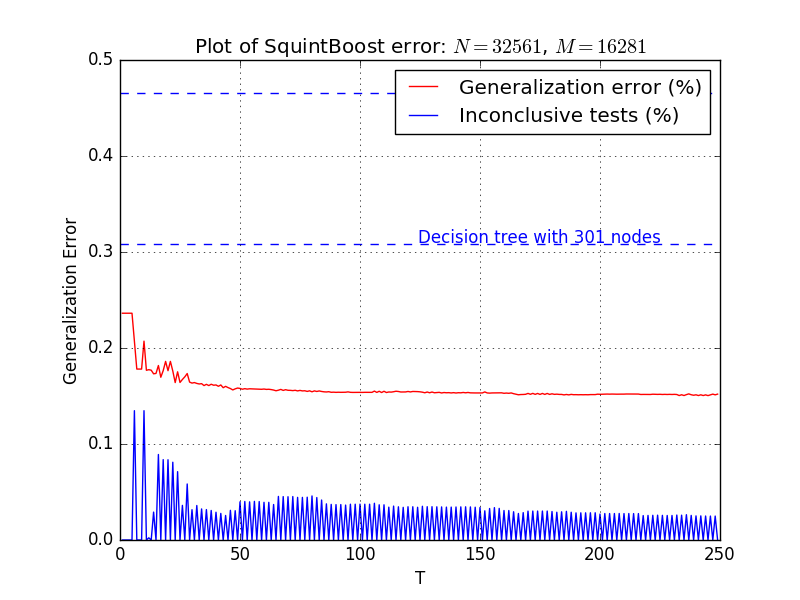
\includegraphics[width=\graphWidth]{generated/SQSVM.png}
  \caption{Generalization error of \squintB as a function of the number of iterations on the a9a data. The error rates of trees with 3 and 385 nodes resp. are again shown for reference. It is important to remark that for clarities' sake we omitted the inconclusive data points of all odd iterations as they are always 0.}
      \label{fig:SQSVM}
\end{figure}
\FloatBarrier
